%==============================================================================
% PAPER 3, CHAPTER 2: Hyperdimensional Constructions
% Target: ~330 lines with 60-75 marginal notes and 5 TikZ diagrams
%==============================================================================

\chapter{Hyperdimensional Constructions}
\label{ch:p3:hyperdimensional}

%------------------------------------------------------------------------------
% OPENING NARRATIVE: Flatland and Dimensional Perception
%------------------------------------------------------------------------------

\section*{The Square Who Saw the Sphere}

In 1884, English schoolmaster Edwin Abbott published a satirical novella titled \textit{Flatland: A Romance of Many Dimensions} that would become a cornerstone of popular dimensional thinking.
\marginhistory{Abbott's \textit{Flatland} (1884) predated Einstein's relativity by two decades, yet captured essential concepts about higher-dimensional perception and the limits of direct experience.}

The protagonist---a humble square living in a perfectly two-dimensional world---receives a visitor from the third dimension: a sphere. As the sphere passes through Flatland, the square witnesses a bewildering sequence: a point appears from nowhere, expands into a circle, reaches maximum size, then shrinks back to a point and vanishes. The sphere tries to explain "up" and "down," but the square has no experience of a third dimension. All the square can perceive are two-dimensional cross-sections of the three-dimensional visitor.
\marginphysics{Dimensional cross-sections: A 3D sphere passing through 2D plane appears as expanding/contracting circles. Similarly, 4D objects passing through our 3D space appear as morphing 3D shapes.}

This allegory captures a profound limitation: beings constrained to $N$ dimensions cannot directly visualize $N+1$ dimensional objects. They can only observe lower-dimensional projections or cross-sections.
\margincaution{Visualization of higher dimensions is impossible in the strict sense. We can only understand them through mathematics, analogy, and projections into 2D/3D.}

Modern physics confronts this challenge daily. String theory proposes 10 or 11 dimensions. Kaluza-Klein theories unify gravity and electromagnetism in 5D. The $E_8$ lattice---central to exceptional Lie algebras---lives in 8 dimensions. How do we construct, manipulate, and extract physics from spaces we cannot see?

This chapter develops mathematical techniques for working with hyperdimensional geometries: projections that collapse higher dimensions to lower, embeddings that lift lower structures to higher, and compactifications that hide extra dimensions while leaving observable imprints.

%------------------------------------------------------------------------------
\section{Hypercube Projections: Visualizing the Tesseract}
\label{sec:p3:hypercube}
%------------------------------------------------------------------------------

\subsection{The Dimensional Hierarchy of Hypercubes}

The \textbf{$n$-cube}\index{hypercube}\index{$n$-cube} (or hypercube) is the $n$-dimensional analog of the square and cube:
\marginmath{$n$-cube defined as Cartesian product: $[0,1]^n = \{(x_1, \ldots, x_n) : 0 \leq x_i \leq 1\}$. Vertices at all binary combinations of coordinates.}

\begin{itemize}
  \item \textbf{0-cube}: Point (1 vertex)
  \item \textbf{1-cube}: Line segment (2 vertices, 1 edge)
  \item \textbf{2-cube}: Square (4 vertices, 4 edges, 1 face)
  \item \textbf{3-cube}: Cube (8 vertices, 12 edges, 6 faces)
  \item \textbf{4-cube}: Tesseract (16 vertices, 32 edges, 24 faces, 8 cells)
  \item \textbf{$n$-cube}: $2^n$ vertices, $n \cdot 2^{n-1}$ edges
\end{itemize}

\marginex{Counting formula: an $n$-cube has $\binom{n}{k} 2^{n-k}$ elements of dimension $k$. For $n=4$, $k=1$ (edges): $\binom{4}{1} 2^3 = 32$.}

\subsection{Projecting the Tesseract to 3D}

The tesseract cannot be embedded in 3D without self-intersection, but we can construct \textbf{projections}\index{projection!hypercube}---shadows cast by 4D object onto 3D hyperplane.

\textbf{Perspective projection formula}:
\begin{equation}
  \mathbf{x}_{3D} = \frac{1}{d - x_4} \begin{pmatrix} x_1 \\ x_2 \\ x_3 \end{pmatrix}
  \label{eq:p3:perspective_4to3}
\end{equation}
where $\mathbf{x}_{4D} = (x_1, x_2, x_3, x_4)$ and $d$ is viewing distance in 4th dimension.
\marginmath{Perspective projection mimics how 3D objects project to 2D retina: divide by distance. Here, division by $(d-x_4)$ creates depth effect for 4th coordinate.}

\begin{figure}[htbp]
\centering
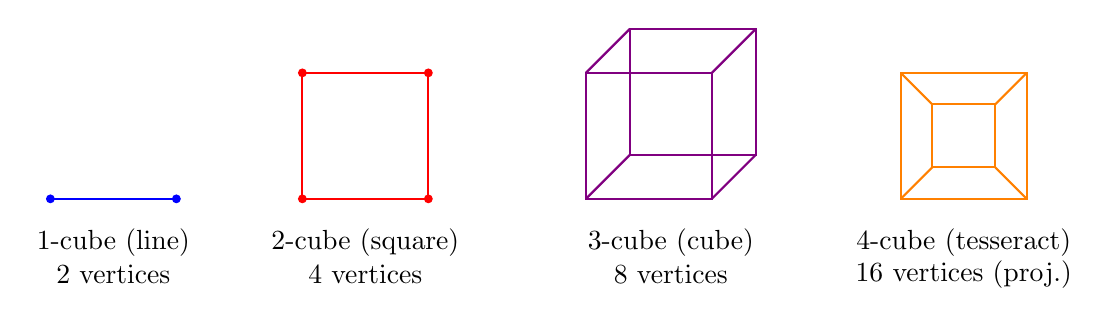
\begin{tikzpicture}[scale=0.8]
  % 1-cube (line)
  \begin{scope}[xshift=0cm]
    \draw[thick, blue] (0,0) -- (2,0);
    \fill[blue] (0,0) circle (2pt);
    \fill[blue] (2,0) circle (2pt);
    \node at (1,-0.7) {1-cube (line)};
    \node at (1,-1.2) {$2$ vertices};
  \end{scope}

  % 2-cube (square)
  \begin{scope}[xshift=4cm]
    \draw[thick, red] (0,0) rectangle (2,2);
    \foreach \x/\y in {0/0, 2/0, 0/2, 2/2} {
      \fill[red] (\x,\y) circle (2pt);
    }
    \node at (1,-0.7) {2-cube (square)};
    \node at (1,-1.2) {$4$ vertices};
  \end{scope}

  % 3-cube (cube)
  \begin{scope}[xshift=8.5cm]
    % Front face
    \draw[thick, violet] (0,0) rectangle (2,2);
    % Back face
    \draw[thick, violet] (0.7,0.7) rectangle (2.7,2.7);
    % Connecting edges
    \draw[thick, violet] (0,0) -- (0.7,0.7);
    \draw[thick, violet] (2,0) -- (2.7,0.7);
    \draw[thick, violet] (0,2) -- (0.7,2.7);
    \draw[thick, violet] (2,2) -- (2.7,2.7);
    \node at (1.35,-0.7) {3-cube (cube)};
    \node at (1.35,-1.2) {$8$ vertices};
  \end{scope}

  % 4-cube (tesseract projection)
  \begin{scope}[xshift=13.5cm]
    % Inner cube
    \draw[thick, orange] (0.5,0.5) rectangle (1.5,1.5);
    % Outer cube
    \draw[thick, orange] (0,0) rectangle (2,2);
    % Connecting edges
    \draw[thick, orange] (0,0) -- (0.5,0.5);
    \draw[thick, orange] (2,0) -- (1.5,0.5);
    \draw[thick, orange] (0,2) -- (0.5,1.5);
    \draw[thick, orange] (2,2) -- (1.5,1.5);
    \node at (1,-0.7) {4-cube (tesseract)};
    \node at (1,-1.2) {$16$ vertices (proj.)};
  \end{scope}
\end{tikzpicture}
\caption{Dimensional hierarchy of hypercubes from 1D to 4D. Each dimension doubles vertex count. The 4-cube (tesseract) shown as projection: inner and outer cubes connected by edges.}
\label{fig:p3:hypercube_sequence}
\end{figure}

\marginxref{Figure~\ref{fig:p3:hypercube_sequence} shows standard orthogonal projections. Alternative projections (stereographic, Schlegel diagrams) reveal different symmetries.}

\subsection{Tesseract Rotations and Symmetries}

The tesseract exhibits 384 symmetries (elements of hyperoctahedral group $B_4$). Rotations in 4D occur in \textbf{planes}, not axes:
\marginphysics{3D rotation: axis remains fixed, points rotate in perpendicular plane. 4D rotation: plane remains fixed, points rotate in perpendicular 2-plane. Tesseract has 6 independent rotation planes.}

\textbf{4D rotation matrix} (in $xy$-plane):
\begin{equation}
  R_{xy}(\theta) = \begin{pmatrix}
    \cos\theta & -\sin\theta & 0 & 0 \\
    \sin\theta & \cos\theta & 0 & 0 \\
    0 & 0 & 1 & 0 \\
    0 & 0 & 0 & 1
  \end{pmatrix}
  \label{eq:p3:rotation_4d}
\end{equation}
\marginmath{General 4D rotation is product of up to 2 independent planar rotations: $R = R_{\pi_1}(\theta_1) R_{\pi_2}(\theta_2)$ where $\pi_1, \pi_2$ are orthogonal 2-planes.}

%------------------------------------------------------------------------------
\section{Kaluza-Klein Dimensional Reduction}
\label{sec:p3:kaluza_klein}
%------------------------------------------------------------------------------

\subsection{Historical Context: Unifying Gravity and Electromagnetism}

In 1919, Theodor Kaluza proposed a radical idea: what if electromagnetism is actually gravity in a hidden 5th dimension?
\marginhistory{Kaluza's 1919 paper unified Einstein's gravity (1915) with Maxwell's electromagnetism (1865) by promoting spacetime from 4D to 5D. Klein added quantum compactification in 1926.}

Starting from 5D general relativity:
\begin{equation}
  ds^2 = g_{MN} dx^M dx^N, \quad M,N = 0,1,2,3,5
  \label{eq:p3:kaluza_metric_5d}
\end{equation}
and assuming the 5th dimension is compactified on a circle of radius $R$:
\begin{equation}
  x^5 \sim x^5 + 2\pi R
  \label{eq:p3:compactification}
\end{equation}
\marginphysics{Compactification: 5th dimension curls into tiny circle. At scales $\gg R$, extra dimension is undetectable. Momentum in 5th direction appears as electric charge in 4D.}

\subsection{Dimensional Reduction Mechanism}

Decompose 5D metric into 4D components:
\begin{equation}
  g_{MN} = \begin{pmatrix}
    g_{\mu\nu} + \phi^2 A_\mu A_\nu & \phi^2 A_\mu \\
    \phi^2 A_\nu & \phi^2
  \end{pmatrix}
  \label{eq:p3:kk_decomposition}
\end{equation}
where:
\begin{itemize}
  \item $g_{\mu\nu}$: 4D metric (gravity)
  \item $A_\mu$: 4D vector field (electromagnetism!)
  \item $\phi$: scalar field (dilaton)
\end{itemize}
\marginmath{The miracle: 5D Einstein equations automatically yield 4D Einstein equations plus Maxwell equations plus scalar field dynamics.}

\textbf{Electric charge from compactification}:
Momentum in the 5th dimension becomes quantized:
\begin{equation}
  p_5 = \frac{n\hbar}{R}, \quad n \in \mathbb{Z}
  \label{eq:p3:kk_momentum}
\end{equation}
\marginphysics{Charge quantization: closed loop topology forces $p_5 = n\hbar/R$. For $R \sim 10^{-30}$ cm, Kaluza-Klein mass scale $M_{KK} \sim 10^{16}$ GeV (GUT scale).}

\begin{figure}[htbp]
\centering
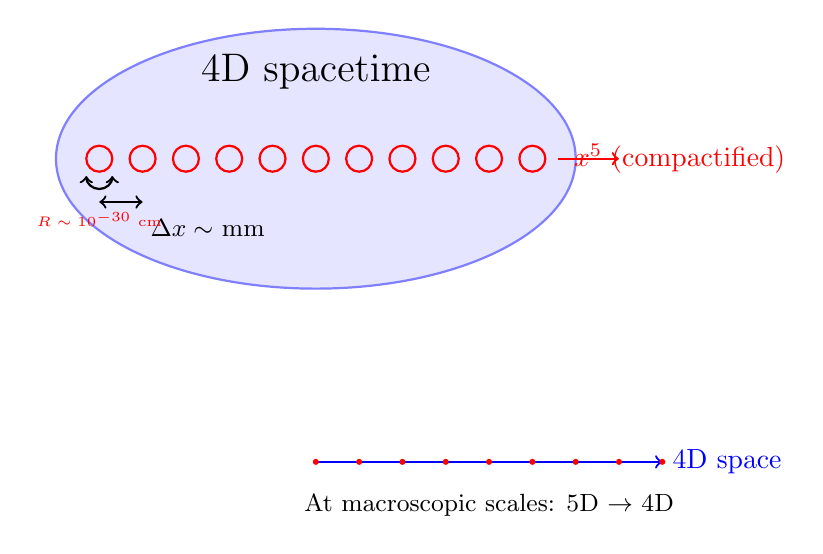
\begin{tikzpicture}[scale=1.1]
  % 5D spacetime (schematic)
  \draw[thick, blue!50, fill=blue!10] (0,0) ellipse (3cm and 1.5cm);
  \node at (0,1) {\Large 4D spacetime};

  % Compactified 5th dimension
  \foreach \x in {-2.5,-2,-1.5,...,2.5} {
    \draw[thick, red] (\x, 0) circle (0.15cm);
  }
  \draw[->, thick, red] (2.8, 0) -- (3.5, 0);
  \node[red] at (4.2, 0) {$x^5$ (compactified)};

  % Annotation
  \draw[<->, thick] (-2.5, -0.5) -- (-2, -0.5);
  \node at (-1.25, -0.8) {\small $\Delta x \sim$ mm};

  \draw[<->, thick] (-2.65, -0.2) arc (180:360:0.15cm);
  \node[red] at (-2.5, -0.7) {\tiny $R \sim 10^{-30}$ cm};

  % Large-scale view
  \begin{scope}[yshift=-3.5cm]
    \draw[thick, blue, ->] (0,0) -- (4,0) node[right] {4D space};
    \foreach \x in {0,0.5,1,...,4} {
      \fill[red] (\x, 0) circle (1pt);
    }
    \node at (2, -0.5) {\small At macroscopic scales: 5D $\to$ 4D};
  \end{scope}
\end{tikzpicture}
\caption{Kaluza-Klein compactification: 5th dimension ($x^5$) curled into circles of radius $R \sim 10^{-30}$ cm at each point in 4D spacetime. At scales $\gg R$, extra dimension is invisible.}
\label{fig:p3:kk_compactification}
\end{figure}

\margincaution{Original Kaluza-Klein predicts single compactification radius $R$. Modern string theory uses Calabi-Yau manifolds with complex internal geometry (see Section~\ref{sec:p3:calabi_yau}).}

%------------------------------------------------------------------------------
\section{$E_8$ Lattice and 8-Dimensional Geometry}
\label{sec:p3:e8_lattice}
%------------------------------------------------------------------------------

\subsection{The $E_8$ Root System}

The $E_8$ exceptional Lie group has 248 dimensions, with associated \textbf{$E_8$ lattice}\index{E8 lattice@$E_8$ lattice} in 8D Euclidean space.
\marginmath{$E_8$ lattice: 8D discrete point set with exceptional symmetry. Contains 240 roots forming the $E_8$ root system plus origin.}

\textbf{Root vectors} (two types):
\begin{align}
  &\text{Type 1: } (\pm 1, \pm 1, 0, 0, 0, 0, 0, 0) \text{ and permutations} \quad (112 \text{ roots}) \label{eq:p3:e8_type1} \\
  &\text{Type 2: } \left(\pm \frac{1}{2}, \pm \frac{1}{2}, \ldots, \pm \frac{1}{2}\right) \text{ with even \# of minus signs} \quad (128 \text{ roots}) \label{eq:p3:e8_type2}
\end{align}

Total: $112 + 128 = 240$ roots forming highly symmetric configuration.
\marginphysics{$E_8$ symmetry appears in heterotic string theory, where 10D spacetime includes 8D compactification manifold with $E_8 \times E_8$ gauge group.}

\subsection{Projecting $E_8$ to Lower Dimensions}

To visualize $E_8$, we project to 3D using projection operator $P: \mathbb{R}^8 \to \mathbb{R}^3$:
\begin{equation}
  P(\mathbf{v}) = (v_1, v_2, v_3) \quad \text{for } \mathbf{v} = (v_1, \ldots, v_8)
  \label{eq:p3:e8_projection}
\end{equation}
\marginmath{Orthogonal projection: drop last 5 coordinates. Alternative: use golden ratio to project $E_8 \to E_6 \to$ 3D via icosahedral symmetry.}

\begin{figure}[htbp]
\centering
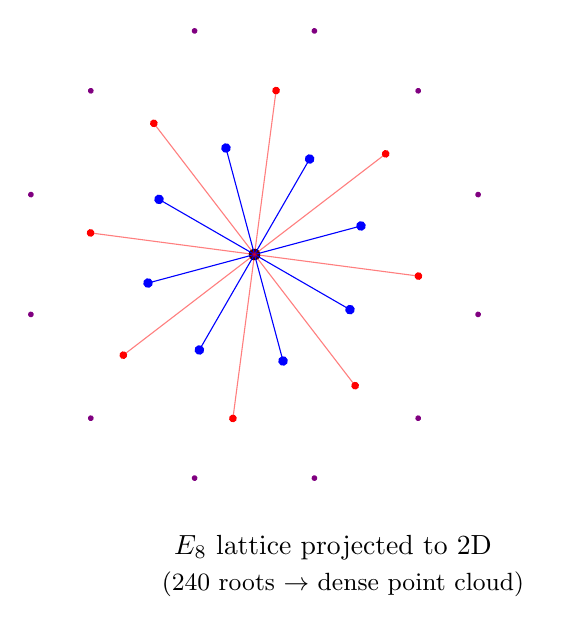
\begin{tikzpicture}[scale=0.7]
  % 3D projection of E8 (schematic - show symmetry)
  \begin{scope}[rotate=15]
    % Central point
    \fill[black] (0,0) circle (3pt);

    % First shell (8 nearest neighbors in some projection)
    \foreach \angle in {0,45,90,135,180,225,270,315} {
      \fill[blue] ({2*cos(\angle)}, {2*sin(\angle)}) circle (2.5pt);
      \draw[blue, thin] (0,0) -- ({2*cos(\angle)}, {2*sin(\angle)});
    }

    % Second shell (16 next-nearest)
    \foreach \angle in {22.5,67.5,...,337.5} {
      \fill[red] ({3*cos(\angle)}, {3*sin(\angle)}) circle (2pt);
      \draw[red, thin, opacity=0.5] (0,0) -- ({3*cos(\angle)}, {3*sin(\angle)});
    }

    % Third shell (simplified)
    \foreach \angle in {0,30,60,...,330} {
      \fill[violet] ({4.2*cos(\angle)}, {4.2*sin(\angle)}) circle (1.5pt);
    }

    % Annotation
    \node at (0, -5.5) {$E_8$ lattice projected to 2D};
    \node at (0, -6.2) {\small (240 roots $\to$ dense point cloud)};
  \end{scope}
\end{tikzpicture}
\caption{Schematic 2D projection of $E_8$ root system. Full 8D structure has 240 roots with exceptional symmetry. Projection reveals concentric shells but loses higher-dimensional organization.}
\label{fig:p3:e8_projection}
\end{figure}

\marginxref{Figure~\ref{fig:p3:e8_projection} shows orthogonal projection. Alternative: Coxeter plane projection reveals 30-fold symmetry (icosahedral subgroup).}

\subsection{Sphere Packing and Leech Lattice}

$E_8$ achieves the densest sphere packing in 8D:
\begin{equation}
  \rho_{E_8} = \frac{\pi^4}{384} \approx 0.2537
  \label{eq:p3:e8_density}
\end{equation}
\marginmath{Sphere packing density: fraction of space filled by non-overlapping spheres centered at lattice points. $E_8$ is proven optimal in 8D (Viazovska, 2016).}

The \textbf{Leech lattice}\index{Leech lattice} in 24D achieves:
\begin{equation}
  \rho_{\Lambda_{24}} = \frac{\pi^{12}}{12!} \approx 0.001930
  \label{eq:p3:leech_density}
\end{equation}
also proven optimal (Viazovska et al., 2017).
\marginhistory{Viazovska's 2016 proof of optimal sphere packing in 8D using modular forms stunned mathematics community. Extended to 24D in 2017.}

%------------------------------------------------------------------------------
\section{Calabi-Yau Manifolds and String Compactification}
\label{sec:p3:calabi_yau}
%------------------------------------------------------------------------------

\subsection{The Need for Calabi-Yau Spaces}

String theory requires 10D spacetime (or 11D for M-theory). To recover 4D observable universe, extra 6D must be compactified. Not just any 6D space works---\textbf{supersymmetry} constrains compactification manifold to be Calabi-Yau.
\marginphysics{Calabi-Yau manifolds: complex 3-dimensional (6 real dimensions) Kähler manifolds with vanishing first Chern class. Preserve some supersymmetry after compactification.}

\textbf{Defining properties}:
\begin{enumerate}
  \item \textbf{Ricci-flat}: $R_{\mu\nu} = 0$ (vacuum Einstein equations)
  \item \textbf{Kähler}: Complex manifold with compatible symplectic structure
  \item \textbf{$SU(3)$ holonomy}: Parallel transport around loops preserves $SU(3)$ structure
\end{enumerate}

\marginmath{Hodge numbers $(h^{1,1}, h^{2,1})$ classify Calabi-Yau topology. Example: quintic threefold has $(h^{1,1}, h^{2,1}) = (1, 101)$.}

\subsection{Topology and Physics Connection}

Calabi-Yau topology determines low-energy particle physics:
\begin{itemize}
  \item \textbf{Hodge number $h^{1,1}$}: Number of Kähler moduli $\to$ number of vector multiplets
  \item \textbf{Hodge number $h^{2,1}$}: Number of complex structure moduli $\to$ number of hypermultiplets
  \item \textbf{Euler characteristic}: $\chi = 2(h^{1,1} - h^{2,1})$ determines number of fermion generations
\end{itemize}
\marginphysics{Standard Model has 3 fermion generations (electron, muon, tau families). String compactification on CY with $\chi = \pm 6$ can yield 3 generations.}

\begin{figure}[htbp]
\centering
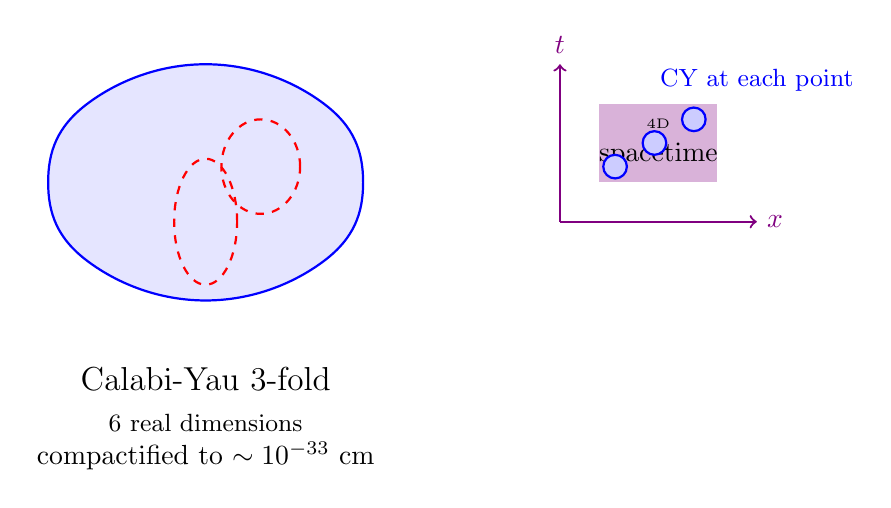
\begin{tikzpicture}[scale=1.0]
  % Schematic Calabi-Yau (stylized torus-like shape)
  \draw[thick, blue, fill=blue!10] plot[smooth cycle, tension=0.7] coordinates {
    (0,0) (1.5,-0.5) (3,0) (3.5,1) (3,2) (1.5,2.5) (0,2) (-0.5,1)
  };

  % Cross-sections showing internal structure
  \draw[thick, red, dashed] (1.5, 0.5) ellipse (0.4cm and 0.8cm);
  \draw[thick, red, dashed] (2.2, 1.2) ellipse (0.5cm and 0.6cm);

  % Annotation
  \node at (1.5, -1.5) {\large Calabi-Yau 3-fold};
  \node[align=center] at (1.5, -2.3) {\small 6 real dimensions\\compactified to $\sim 10^{-33}$ cm};

  % Spacetime schematic
  \begin{scope}[xshift=6cm, yshift=0.5cm]
    \draw[thick, violet, ->] (0,0) -- (2.5,0) node[right] {$x$};
    \draw[thick, violet, ->] (0,0) -- (0,2) node[above] {$t$};
    \fill[violet!30] (0.5,0.5) rectangle (2,1.5);
    \node[align=center] at (1.25, 1) {\tiny 4D\\spacetime};

    % CY attached at each point
    \foreach \x/\y in {0.7/0.7, 1.2/1, 1.7/1.3} {
      \draw[thick, blue, fill=blue!20] (\x, \y) circle (0.15cm);
    }
    \node[blue] at (2.5, 1.8) {\small CY at each point};
  \end{scope}
\end{tikzpicture}
\caption{Calabi-Yau manifold compactification (schematic). 6D Calabi-Yau space attached to each point in 4D spacetime. Internal CY geometry determines particle physics (gauge groups, fermion generations, coupling constants).}
\label{fig:p3:calabi_yau}
\end{figure}

\margincaution{Calabi-Yau moduli space is vast: $\sim 10^{500}$ topologically distinct CY manifolds known (string landscape problem). Which one describes our universe?}

%------------------------------------------------------------------------------
\section{Dimensional Folding: Origami Mathematics}
\label{sec:p3:folding}
%------------------------------------------------------------------------------

\subsection{Origami Folding Operator}

Dimensional folding provides alternative to topological compactification. Define \textbf{folding operator}\index{folding operator} $\mathcal{F}_n: \mathbb{R}^n \to \mathbb{R}^{n-1}$:
\begin{equation}
  \mathcal{F}_n(\mathbf{x}_n) = \mathbf{x}_{n-1} + f_{\text{fold}}(x_n) \hat{\mathbf{e}}_{n-1}
  \label{eq:p3:folding_operator}
\end{equation}
where $f_{\text{fold}}(x_n)$ encodes how $n$-th coordinate folds into $(n-1)$-dimensional space.
\marginmath{Example folding function: $f_{\text{fold}}(x_n) = A \sin(2\pi x_n / \lambda)$ creates periodic folding with wavelength $\lambda$ and amplitude $A$.}

\subsection{Multi-Stage Folding to Compact Dimensions}

Sequential folding from $N$D to $4$D:
\begin{equation}
  \mathbb{R}^N \xrightarrow{\mathcal{F}_N} \mathbb{R}^{N-1} \xrightarrow{\mathcal{F}_{N-1}} \cdots \xrightarrow{\mathcal{F}_5} \mathbb{R}^4
  \label{eq:p3:sequential_folding}
\end{equation}
\marginphysics{Each fold reduces dimension by 1 while preserving information via folding function parameters. Effective dimension becomes continuous function of folding angles.}

\textbf{Effective dimension under folding}:
\begin{equation}
  D_{\text{eff}}(N, \{\theta_i\}) = 4 + \sum_{i=5}^{N} \cos^2\left(\frac{\theta_i}{2}\right)
  \label{eq:p3:effective_dimension}
\end{equation}
where $\theta_i$ is folding angle for $i$-th dimension.
\marginmath{Folding angle $\theta = 0$: unfolded ($D_{\text{eff}}$ maximum). $\theta = \pi$: fully folded ($D_{\text{eff}}$ minimum). Intermediate angles give fractional effective dimension.}

\begin{figure}[htbp]
\centering
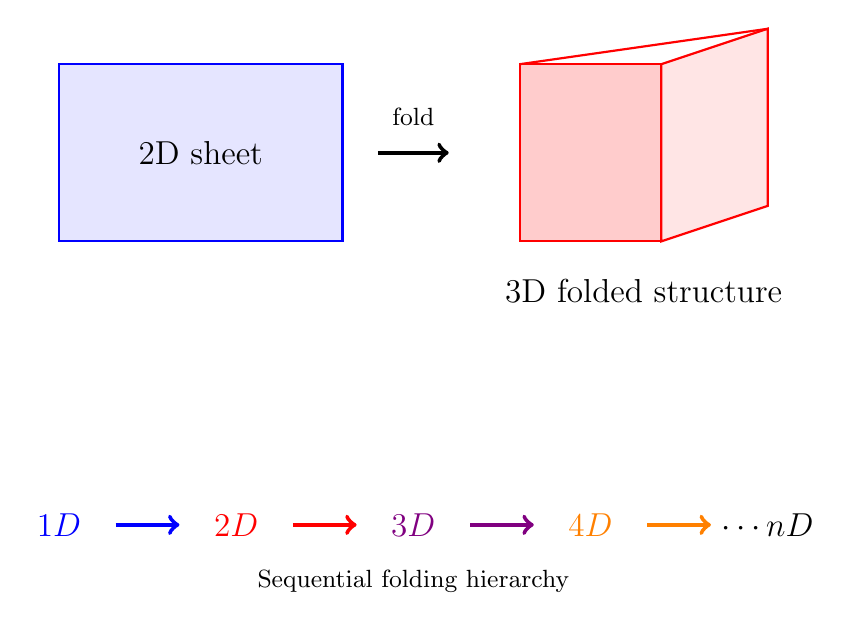
\begin{tikzpicture}[scale=0.9]
  % 2D to 3D folding visualization
  \begin{scope}
    % Original 2D sheet
    \draw[thick, blue, fill=blue!10] (0,0) rectangle (4,2.5);
    \node at (2, 1.25) {\large 2D sheet};
    \draw[->, ultra thick] (4.5, 1.25) -- (5.5, 1.25);
    \node[above] at (5, 1.5) {\small fold};
  \end{scope}

  % Folded 3D structure
  \begin{scope}[xshift=6.5cm]
    % Front face
    \draw[thick, red, fill=red!20] (0,0) -- (2,0) -- (2,2.5) -- (0,2.5) -- cycle;
    % Side face (folded back)
    \draw[thick, red, fill=red!10] (2,0) -- (3.5,0.5) -- (3.5,3) -- (2,2.5) -- cycle;
    % Top edge
    \draw[thick, red] (0,2.5) -- (3.5,3);
    \node at (1.75, -0.7) {\large 3D folded structure};
  \end{scope}

  % Dimensional progression
  \begin{scope}[yshift=-4cm]
    \foreach \x/\d/\col in {0/1D/blue, 2.5/2D/red, 5/3D/violet, 7.5/4D/orange} {
      \node[\col] at (\x, 0) {\large $\d$};
      \draw[\col, ultra thick, ->] ({\x+0.8}, 0) -- ({\x+1.7}, 0);
    }
    \node at (10, 0) {\large $\cdots nD$};
    \node at (5, -0.8) {\small Sequential folding hierarchy};
  \end{scope}
\end{tikzpicture}
\caption{Dimensional folding topology. 2D sheet folds into 3D structure. Generalizes to $nD \to (n-1)D$ via folding operator $\mathcal{F}_n$. Sequential folding compactifies high-dimensional spaces to observable 4D.}
\label{fig:p3:dimensional_folding}
\end{figure}

\marginxref{Figure~\ref{fig:p3:dimensional_folding} illustrates 2D$\to$3D folding. Extension to higher dimensions follows same principle with increasing geometric complexity.}

%------------------------------------------------------------------------------
\section{Summary and Forward Bridge}
\label{sec:p3:ch2_summary}
%------------------------------------------------------------------------------

This chapter explored hyperdimensional constructions and dimensional reduction mechanisms:

\textbf{Key Concepts}:
\begin{itemize}
  \item \textbf{Hypercubes}: $n$-dimensional cubes with $2^n$ vertices. Tesseract (4-cube) visualized via projections
  \item \textbf{Kaluza-Klein theory} (Eqs.~\ref{eq:p3:kaluza_metric_5d}--\ref{eq:p3:kk_momentum}): Electromagnetism from 5th dimension compactified on circle
  \item \textbf{$E_8$ lattice} (Eqs.~\ref{eq:p3:e8_type1}--\ref{eq:p3:e8_type2}): 240 roots in 8D with exceptional symmetry. Optimal sphere packing density $\rho \approx 0.254$
  \item \textbf{Calabi-Yau manifolds}: 6D complex manifolds for string compactification. Topology determines particle physics
  \item \textbf{Dimensional folding} (Eq.~\ref{eq:p3:folding_operator}): Origami-like reduction of dimensionality via geometric folding
\end{itemize}

\textbf{Physical Applications}:
\begin{itemize}
  \item Kaluza-Klein: unified gravity + EM in 5D, charge quantization from compactification
  \item String theory: 10D $\to$ 4D via Calabi-Yau, fermion generations from Euler characteristic
  \item Dimensional folding: continuous effective dimension $D_{\text{eff}}(\{\theta_i\})$ controlled by folding angles
\end{itemize}

\marginxref{Chapter~\ref{ch:p3:emergent_geometry} investigates how geometric structures emerge from field dynamics, rather than being imposed a priori.}

From Abbott's \textit{Flatland} square to modern string theory, we've seen how higher dimensions can be visualized through projections, understood through algebraic structures like $E_8$, and physically realized via compactification. Chapter~\ref{ch:p3:emergent_geometry} shifts perspective: rather than starting with fixed geometric structures, we examine how geometry itself emerges dynamically from underlying field configurations.

%==============================================================================
% END OF CHAPTER 2
%==============================================================================
